\section{Gestión de carteras}



\subsection{Carteras diversificadas}
Se tiene una cartera con $N$ activos. El valor hoy del i-ésimo activo es $S_i$ y tiene un retorno aleatorio $R_i$ sobre el periodo $T$. Los retornos están distribuidos de forma normal con media $\mu_i T$ y varianza $\sigma_i\sqrt{T}$. La correlación entre los activos $i$ y $j$ es $\rho_{ij}$. Se tiene una cantidad $w_i$ del activo $i$ en la cartera, por lo que
\begin{align*}
    \Pi &= \sum_{i=1}^N w_i S_i \Rightarrow \\
    \Rightarrow \delta\Pi &= \sum_{i=1}^N w_i R_i S_i \Rightarrow \\
    \Rightarrow \frac{\delta\Pi}{\Pi} &= \frac{\sum_{i=1}^N w_i R_i S_i}{\sum_{i=1}^N w_i S_i} \\
    &= \sum_{i=1}^N W_i R_i, \qquad W_i = \frac{w_i S_i}{\sum_{j=1}^N w_j S_j} \\
\end{align*}
por lo que el retorno esperado de la cartera es
\begin{align}\label{eq:esperanza_cartera}
    \mu_{\Pi} &= \frac{1}{T}\mathbb{E}\left[\frac{\delta\Pi}{\Pi}\right] = \frac{1}{T}\mathbb{E}\left[\sum_{i=1}^N W_i R_i\right] = \frac{1}{T} \sum_{i=1}^N W_i \mathbb{E}[R_i] = \frac{1}{T} \sum_{i=1}^N W_i \mu_i T \nonumber \\
    &= \boxed{\sum_{i=1}^N W_i \mu_i}
\end{align}
y la desviación estandar
\begin{equation}\label{eq:desviacion_cartera}
    \sigma_{\Pi} = \frac{1}{\sqrt{T}}\sqrt{\text{var}\left[ \frac{\delta\Pi}{\Pi} \right]} = \boxed{\sqrt{\sum_{i=1}^N \sum_{j=1}^N W_i W_j \rho_{ij} \sigma_i \sigma_j}}
\end{equation}
siendo
\[
    \boxed{W_i = \frac{w_i S_i}{\sum_{j=1}^N w_j S_j}}
\]
y sabiendo que
\[
    \sum_{i=1}^N W_i = 1.
\]

En estos contextos, a la volatilidad o desviación típica se le llama \textbf{risk} y a rentabilidad esperada se le llama \textbf{return}.





\subsection{Elección de activos dentro de una cartera diversificada: modelo de Markowitz (MPT)}
Se va a definir las carteras de manera que sean eficientes, que son aquellas que dan el mayor reward dado un novel de risk o que el menor risk dado un nivel de reward. 

Por ejemplo, se tiene que elegir una cartera que combine dos activos $A$ y $B$. Usando las ecuaciones~\eqref{eq:esperanza_cartera} y~\eqref{eq:desviacion_cartera}, se tiene que
\begin{align*}
    \mu_\Pi &= W \mu_A + (1 - W) \mu_B \\
    \sigma^2_\Pi &= W^2 \sigma_A^2 + 2W(1-W)\rho_{AB}\sigma_A\sigma_B + (1-W)^2 \sigma_B^2
\end{align*}
Lo que da la siguiente curva:
\begin{figure}[H]
    \centering
    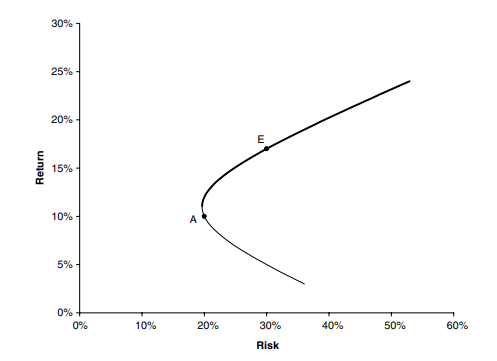
\includegraphics[width=0.65\linewidth]{Imagenes/Parte1/14_Gestion_carteras/Combinacion_activos.png}
    \caption{Combinación de activos en una cartera}
\end{figure}
la mejor opción en este caso es elegir un $W$ para encontrarse dentro de la \textbf{efficient frontier} (parte en negrita de la curva), según el nivel de riesgo que se quiera asumir. Dependiendo del lugar en la curva, se debe tener una posición long o short de los activos.


También se puede añadir un activo libre de riesgo con un retorno $r$, como sería el activo $F$ en la siguiente figura:
\begin{figure}[H]
    \centering
    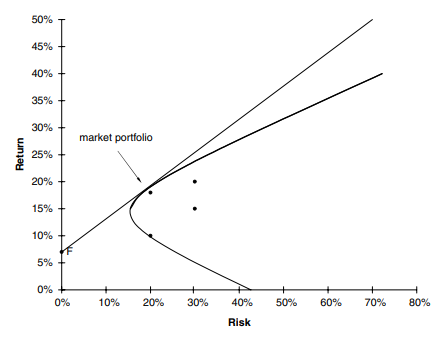
\includegraphics[width=0.65\linewidth]{Imagenes/Parte1/14_Gestion_carteras/Combinacion_activos_Free_Risk.png}
    \caption{Combinación de activos en una cartera con activo libre de riesgo}
    \label{fig:cartera_free_risk}
\end{figure}
Este nuevo activo da una nueva frontera eficiente que es una línea recta llamada \textbf{Capital Market Line} (CML) y el punto con el que toca la frontera eficiente original se llama \textbf{Market Portfolio}.




La elección de activos dentro de la frontera eficiente es subjetiva y depende del riesgo que se quiera asumir, pero hay maneras de interpretar el risk/reward. 

Se compra $\alpha$ ``unidades'' de la cartera $\Pi$ y $(1-\alpha)$ del activo libre de riesgo, por lo que el nuevo retorno esperado es
\[
    \mu = \alpha \mu_{\Pi} + (1 - \alpha) r = r + \alpha \left( \mu_{\Pi} - r \right)
\]
y la nueva desviación estándar es
\[
    \sigma = \alpha \sigma_{\Pi}
\]
por lo que
\[
    \mu = r + \frac{\sigma}{\sigma_{\Pi}} \left( \mu_{\Pi} - r \right)
\]
es decir
\[
    \mu = r + s \sigma, \qquad \boxed{s = \frac{\mu_{\Pi} - r}{\sigma_{\Pi}}}
\]

EL valor $s$ es una medida de probabilidad de que la rentabilidad de la cartera sea mayor que $r$. Sea $C(\cdot)$ la función de distribución acumulada de la normal (se asume que el retorno de la cartera $\Pi$ sigue una normal, por lo que también lo siguen $\mu_{\Pi}$ y $\sigma_{\Pi}$), entonces $C(s)$ es la probabilidad de que el retorno de la cartera sea mayor que $r$. Por lo que si se quiere minimizar la probabilidad de que el retorno sea menor que $r$, se debe elegir una cartera $\Pi_{\text{eff}}$ dentro de la frontera eficiente con la mayor pendiente
\[
    \frac{\mu_{\text{eff}} -  r}{\sigma_{\text{eff}}}
\]

Si se consigue mantener la pentiente de la recta de la figura~\ref{fig:cartera_free_risk}, se puede decir con una confianza $C(s)$ que la cartera no perderá más de
\[
    \mu_{\text{eff}} - s \sigma_{\text{eff}}
\]
por lo que el objetivo es elegir una cartera que maximice esa cantidad.

Un problema del modelo de Markowitz es que necesita muchos parámetros de entrada.






\subsection{Capital Asset Pricing Model (CAPM)}
En primer lugar, se define \textbf{beta} de un activo con respecto a una cartera $M$ como el ratio entre la covarianza entre el retorno del activo y el rendimiento en la cartera por la varianza de la cartera
\[
    \beta_i = \frac{\text{cov}(R_i, R_M)}{\text{var}(R_M)} 
\]

De forma intuitiva, mide cuánto se mueve el activo en promedio cuando la cartera o el mercado se mueve.
\begin{table}[H]
    \centering
    \begin{tabular}{|c|l|}
        \hline
        \textbf{Valor de \( \beta_i \)} & \textbf{Interpretación} \\
        \hline
        \( \beta_i = 1 \) & El activo se mueve igual que el mercado. \\
        \hline
        \( \beta_i > 1 \) & El activo es más volátil que el mercado (más riesgoso, mayor retorno esperado). \\
        \hline
        \( \beta_i < 1 \) & El activo es más defensivo: se mueve menos que el mercado. \\
        \hline
        \( \beta_i = 0 \) & El activo no tiene relación con el mercado (ej.:\ bono de corto plazo). \\
        \hline
        \( \beta_i < 0 \) & El activo se mueve en dirección contraria al mercado (activo refugio). \\
        \hline
    \end{tabular}
\end{table}

Se va a contruir ahora un \textbf{single-index model}, que realciona la rentabilidad de todos los activos a la rentabilidad de un índice representativo $M$. Se escribe el retorno del i-ésimo activo como
\[
    R_i = \alpha_i + \beta_i R_M + \epsilon_i
\]
por lo que el retorno de un activo se puede descomponer en un drift constante ($\alpha_i$), una parte aleatoria común con el índice $M$ ($\beta_i R_M$) y una parte aleatoria ($\epsilon_i$) no correlada con el índice. Esta parte aleatoria no correlada es única para cada activo y tiene media cero.

EL retorno esperado del i-ésimo activo es
\[
    \mu_i = \alpha_i + \beta_i \mu_M
\]
y la desviación estandar es
\[
    \sigma_i = \sqrt{\beta_i^2 \sigma_M^2 + e_i^2}
\]
siendo $e_i$ la desviación estandar de $\epsilon_i$. Por lo tanto el retorno de una cartera con estos activos es
\[
    \frac{\delta\Pi}{\Pi} = \sum_{i=1}^N W_i R_i = \left( \sum_{i=1}^N W_i a_i \right) + R_M \left( \sum_{i=1}^N W_i \beta_i \right) + \sum_{i=1}^N W_i \epsilon_i
\]
por lo que
\begin{align*}
    \mu_{\Pi} &= \left( \sum_{i=1}^N W_i a_i \right) + \mathbb{E}\left[R_M\right] \left( \sum_{i=1}^N W_i \beta_i \right) \\
    &= \alpha_{\Pi} + \beta_{\Pi} \mathbb{E}\left[R_M\right] = \boxed{\alpha_{\Pi} + \beta_{\Pi} \mu_M}
\end{align*}
siendo
\[
    \alpha_{\Pi} = \sum_{i=1}^N W_i a_i, \qquad \beta_{\Pi} = \sum_{i=1}^N W_i \beta_i
\]

Por otro lado el riesgo de la cartera es
\[
    \boxed{\sigma_{\Pi} = \sqrt{\sum_{i=1}^N \sum_{j=1}^N W_i W_j \beta_i \beta_j \sigma_M^2+ \sum_{i=1}^N W_i^2 e_i^2}}
\]


Si los pesos son todos parecidos (i.e.\ en torno a $1/N$), los términos finales de la raíz son $\mathbb{O}(N^{-1})$ por lo que cuando $N \to \infty$
\[
    \sigma_{\Pi} = \left| \sum_{i=1}^N \sum_{j=1}^N W_i W_j \right|\sigma_M = \left| \beta_{\Pi} \right|\sigma_M
\]
Es decir, a medida que se incremementa el número de activos en la cartera, la contribución de la parte aleatoria no correlada con el índice se vuelve despreciable. El riesgo asociado a $\epsilon$ se le llama \textbf{diversifiable risk} y el correlato al índice \textbf{systematic risk}.

El problema de elección de una cartera es la misma que la de Markowitz, pero son necesarios muchos menos parámetros.



Este modelo se puede extender a un \textbf{multi-index model} en el que se relacionan los activos con varios índices representativos. En este caso, el retorno del i-ésimo activo se escribe como
\[
    R_i = \alpha_i + \sum_{j=1}^n \beta_{ij} R_j + \epsilon_i
\]
donde hay $n$ índices con retorno $R_j$. Los índices pueden estar correlados entre sí. 



Existen otros modelos más avanzados que involucran la \textbf{cointegridad} que no se van a explicar.







\subsection{Medición del desempeño}
AL medir el desempeño de una cartera, no solo es importante que el retorno sea alto, si no que también se haya producido con la mejor aleatoriedad posible (no haya sido suerte). Para ello se usan los siguientes indicadores:
\begin{align*}
    \textbf{Sharpe Ratio} &= \boxed{\frac{\mu_{\Pi} - r}{\sigma_{\Pi}}} \\
    \textbf{Treynor Ratio} &= \boxed{\frac{\mu_{\Pi} - r}{\beta_{\Pi} \sigma_M}}
\end{align*}
donde $\mu_{\Pi}$ y $\sigma_{\Pi}$ son el retorno desviación estándar real de la cartera y $\beta_{\Pi}$ es la medida de la volatilidad de la cartera. El Sharpe ratio se utiliza generalmente cuando la cartera abarca la totalidad de la inversión, y el Treynor ratio, cuando se examina el rendimiento de un componente de la cartera completa de la empresa, por ejemplo. Cuando la cartera en cuestión está altamente diversificada, ambas medidas son iguales (hasta un factor de la desviación estándar del mercado).








